\chapter{Motivazioni e Stato dell'arte}\label{ch:motivations}

  Come detto nell'\nameref{ch:intro}, il rapido aumento di dispositivi capaci di computare e distribuiti nell'ambiente ha reso necessario ideare nuovi paradigmi di programmazione.
  Uno di questi è senza dubbio l'\emph{aggregate programming}, di cui si è trattato nel dettaglio nel~\Cref{ch:aggregate}.
  Prima di partire con la progettazione del sistema, è stato necessario valutare lo stato dell'arte nel quale il software va ad inserirsi.
  In particolare, si è preso in considerazione la procedura di configurazione di un progetto realizzato in un linguaggio aggregato,
  confrontandolo con l'esperienza di sviluppo ottenuta con altri linguaggi in altri contesti.

  In questo \nameCref{ch:motivations} verrà analizzato lo stato dell'arte relativamente alla creazione di un programma aggregato,
  mettendo in evidenza le ragioni per la quale è stato realizzato questo progetto di tesi.

  \section{Accessibilità allo sviluppo in Protelis}\label{subsec:setup}

  I due principali linguaggi di programmazione aggregata che implementano il modello teorico del field calculus sono Protelis e ScaFi.
  ScaFi è un DSL interno a Scala e, come tale, richiede di essere utilizzato all'interno di progetti basati su tale linguaggio;
  poiché sono già state realizzate tesi~\cite{amslaurea12188,amslaurea16824} incentrate sull'esecuzione di ScaFi,
  è stato richiesto di concentrarsi, in questa tesi, solamente su Protelis.

  Protelis è un linguaggio \emph{Java-hosted} e, come tale, deve essere caricato in un progetto JVM che esegue un'istanza del suo interprete.
  Di seguito sono riportate le possibili modalità di esecuzione documentate nello stato dell'arte.

  \begin{description}
    \item[Alchemist]\cite{ProtelisSAC14}
      Una prima possibilità di utilizzo è tramite il simulatore Alchemist~\cite{alchemist-jos2013}.
      Esso mette infatti a disposizione all'interno del proprio meta-modello un'incarnazione specifica per Protelis.
      Esso permette la simulazione di reti con pattern anche complessi con semplici file di configurazione.
      In~\Cref{fig:alchemis-protelis} sono riportate le entità in gioco.

      \begin{figure}[htbp]
        \centering
        \includesvg[width=0.52\textwidth]{res/fig/protelis-alchemist-arch.svg}%
        \caption[
          Implementazione dell'architettura di Protelis in Alchemist
        ]{
          Implementazione dell'architettura di Protelis in Alchemist.

          \nameCref{fig:alchemis-protelis} ripresa da~\cite{ProtelisSAC14}.
        }%
        \label{fig:alchemis-protelis}
      \end{figure}

      Alchemist può essere utilizzato all'interno di altro software in ambiente Java come libreria di virtualizzazione, oppure in modo indipendente tramite linea di comando\footnote{\url{https://github.com/Protelis/Protelis-Alchemist-tutorial}}.
      In questo secondo caso, è possibile definire il codice Protelis insieme a file di configurazione in formato YAML e specificarli al lancio del file jar eseguibile di Alchemist.
      Il simulatore mette a disposizione un'interfaccia grafica minimale per la visualizzazione e il controllo della simulazione.

    \item[ProtelisVM]\cite{amslaurea19778}
      Un'altra possibilità è tramite l'importazione del framework di Protelis nel \emph{classpath} di un progetto Java, ad esempio prelevandolo come dipendenza Maven.
      Il framework mette a disposizione una classe denominata \texttt{ProtelisVM} (\Cref{fig:protelisvm}), che si occupa di eseguire un programma Protelis in un \texttt{ExecutionContext},
      ossia un'astrazione del dispositivo esecutore che si frappone tra la macchina virtuale e l'ambiente fisico.

      \begin{figure}[htbp]
        \centering
        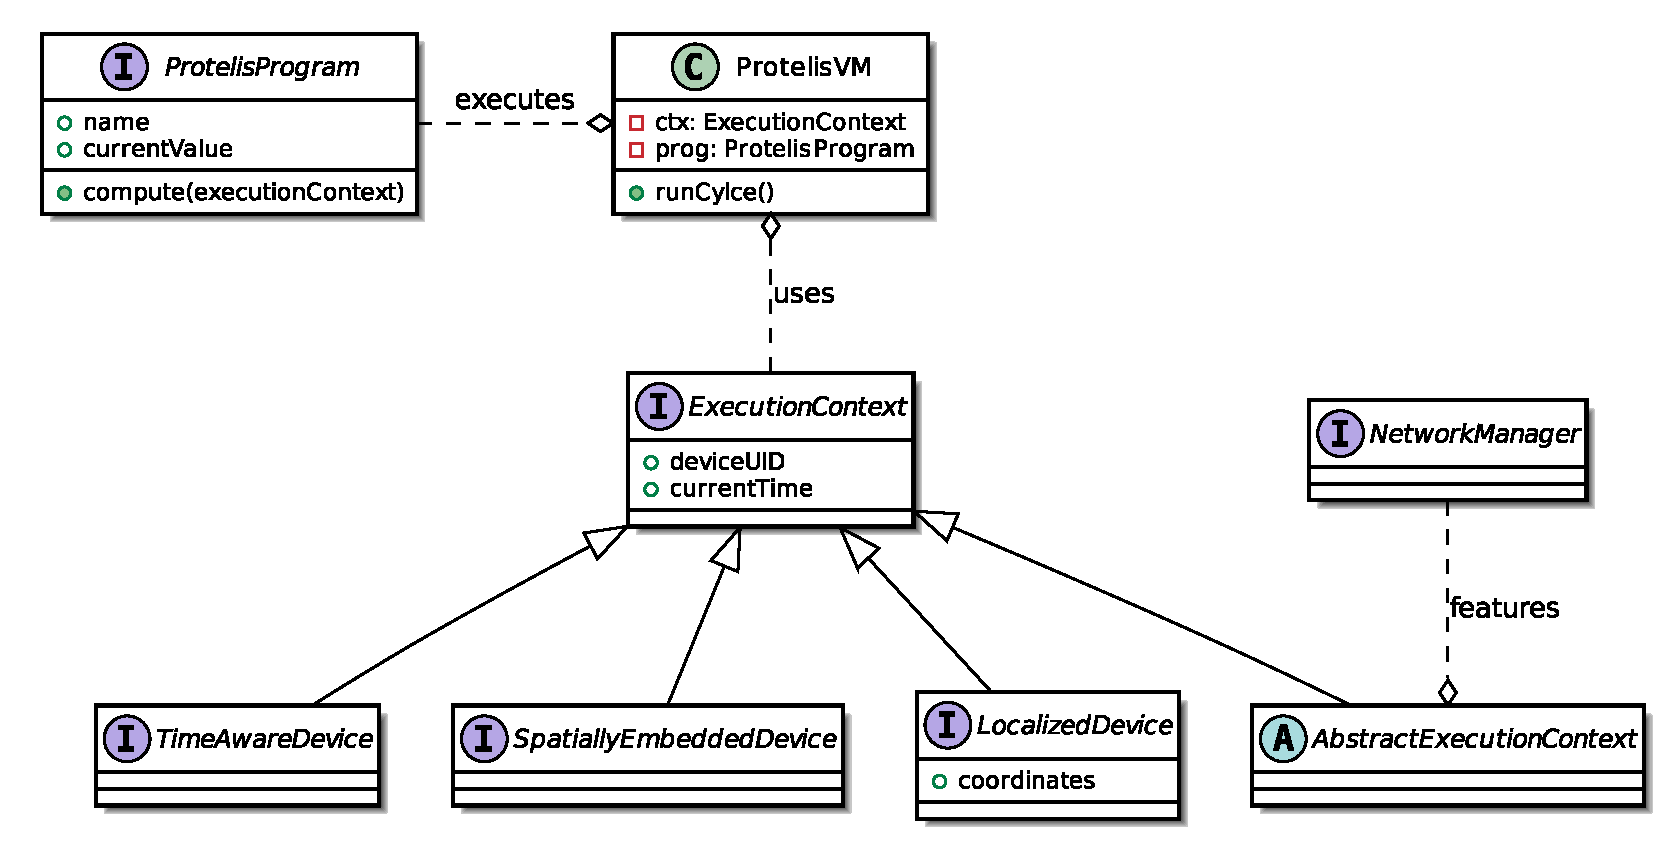
\includegraphics[width=0.87\textwidth]{res/uml/ExecutionContext.eps}%
        \caption{UML delle principali entità del framework di Protelis}%
        \label{fig:protelisvm}
      \end{figure}

      Attraverso la libreria è possibile definire dispositivi virtuali o, potenzialmente, collegare implementazioni fisiche.
      Su GitHub\footnote{\url{https://github.com/Protelis/Protelis-Demo}} sono riportati alcuni esempi con diverse opzioni di integrazione.

    \item[NASA WorldWind]\cite{4161692}
      Un'ultima possibilità vede invece l'utilizzo del framework di visualizzazione open-source WorldWind, sviluppato dalla NASA\@.
      Esso è stato utilizzato per dimostrare come Protelis possa essere uno strumento che permette di controllare anche dispositivi reali come uno sciame di droni.
      Il codice della demo è pubblico su GitHub\footnote{\url{https://github.com/Protelis/Protelis-Demo-Visualized}}.
  \end{description}

  In ciascuno di questi esempi risulta evidente che la configurazione di un progetto per Protelis, anche estremamente minimale, coinvolge strumenti esterni la cui complessità può non essere banale.
  Sarebbe interessante avere a disposizione un ambiente di sviluppo che non richieda configurazione e permetta di provare prototipi di codice durante l'apprendimento del linguaggio.

  \section{Ambienti di sviluppo online}\label{subsec:online-ide}

  Con il progredire delle capacità delle applicazioni JavaScript per browser e della popolarità del linguaggio stesso, sono nate numerose implementazioni di IDE (\emph{Integrated Development Environment}) in grado di eseguire all'interno di una pagina web, comunicando al più con un \emph{language server} remoto.

  Inizialmente sono stati appannaggio di ambienti per la prototipazione di codice JavaScript, in quanto si avvalevano del motore nativamente integrato nel browser per l'esecuzione;
  attualmente molti linguaggi offrono un ambiente di questo tipo, spesso chiamato \emph{playground}, in cui sperimentare (ad esempio Kotlin, TypeScript o Scala).
  Alcuni ambienti di questo tipo, addirittura, sono in grado di offrire un'esperienza utente tanto immediata e completa che talvolta vengono preferite da alcuni a installazioni desktop tradizionali.
  È questo il caso, ad esempio, di Overleaf.

  \emph{Overleaf}\footnote{\url{https://www.overleaf.com}} è un editor per \LaTeX{} completamente online che permette all'utente di scrivere documenti tramite browser;
  il sorgente del markup viene compilato in modo trasparente all'utente, il quale deve preoccuparsi unicamente del contenuto che sta scrivendo.
  Questo risparmia agli utenti inesperti la fase di installazione e configurazione di una distribuzione \LaTeX{} e la scelta di un editor tra i tanti disponibili.

  Potrebbe essere interessante offrire all'utente novizio di Protelis un'esperienza simile:
  la rete di dispositivi (reale o simulata) viene configurata nel server, insieme all'interprete per il linguaggio.
  L'utente avrebbe dunque a disposizione, tramite il proprio browser, solo un semplice editor per scrivere il codice e metterlo in esecuzione.
